\chapter{Phương pháp và mô hình nghiên cứu}
\label{chuong:phuong-phap}

Bài báo của Kassem~\cite{kassem2022} kết hợp ba lớp phân tích trên cùng một bộ dữ liệu khảo sát 314 phiếu: chỉ số tầm quan trọng tương đối (RII) để xếp hạng từng yếu tố rủi ro, ma trận xác suất -- tác động (PIM) để phân vùng rủi ro, và mô hình phương trình cấu trúc bình phương tối thiểu riêng phần (PLS-SEM) để đo ảnh hưởng của các nhóm rủi ro lên thành công dự án. Chương này trình bày cơ sở lý thuyết, công thức và cách đọc kết quả của từng phương pháp.

\section{Dữ liệu khảo sát và độ tin cậy thang đo}
\label{sec:du-lieu}

Dữ liệu của bài báo được thu thập bằng bảng hỏi gồm tám phần. Mỗi yếu tố rủi ro được người trả lời chấm \textbf{hai lần} trên thang Likert 5 mức (1 = rất thấp, 5 = rất cao): một lần cho \emph{xác suất xảy ra} và một lần cho \emph{mức tác động}. Phần cuối hỏi về năm hậu quả của rủi ro đối với dự án. Có 360 phiếu được phát ra, thu về 323 và giữ lại 314 phiếu hợp lệ. Danh sách yếu tố rủi ro ban đầu gồm 61 yếu tố, sau khảo sát thử và tham vấn bốn chuyên gia còn lại 51 yếu tố~\cite{kassem2022}.

Trước khi phân tích, cần kiểm tra các câu hỏi trong cùng một nhóm có đo cùng một khái niệm hay không. Chỉ số thường dùng là hệ số Cronbach's alpha~\cite{cronbach1951}:
\begin{equation}
\alpha = \frac{K}{K-1}\left(1 - \frac{\sum_{i=1}^{K}\sigma_i^2}{\sigma_T^2}\right)
\label{eq:cronbach}
\end{equation}
trong đó $K$ là số câu hỏi của nhóm, $\sigma_i^2$ là phương sai của câu thứ $i$ và $\sigma_T^2$ là phương sai của tổng điểm. Hệ số $\alpha$ càng gần 1 thì các câu hỏi càng nhất quán. Ngưỡng chấp nhận phổ biến là $\alpha \geq 0{,}7$~\cite{hair2019report}. Trong bài báo, cả 13 nhóm rủi ro và nhóm hậu quả đều đạt, với $\alpha$ từ 0,771 đến 0,944.

\section{Chỉ số tầm quan trọng tương đối (RII)}
\label{sec:rii}

\subsection{Công thức}

RII là cách quy đổi điểm Likert của nhiều người trả lời thành một con số duy nhất trong khoảng $(0;1]$ để xếp hạng các yếu tố. Đây là chỉ số được dùng rộng rãi trong các nghiên cứu về chậm tiến độ và vượt chi phí trong xây dựng~\cite{sambasivan2007}:
\begin{equation}
RII = \frac{\sum W}{A \times N} = \frac{\sum_{k=1}^{5} k \cdot n_k}{A \times N}
\label{eq:rii}
\end{equation}
trong đó $W$ là điểm mỗi người trả lời chấm cho yếu tố ($1$ đến $5$), $n_k$ là số người chấm mức $k$, $A = 5$ là điểm cao nhất của thang đo và $N$ là tổng số người trả lời. Giá trị nhỏ nhất của RII là $1/5 = 0{,}2$ (mọi người đều chấm 1) và lớn nhất là 1 (mọi người đều chấm 5).

\emph{Lưu ý:} bài báo định nghĩa $W$ là ``điểm trung bình có trọng số của người trả lời, nhận giá trị từ 1 đến 5''~\cite{kassem2022}. Nếu $W$ là điểm trung bình thì không được chia thêm cho $N$, vì làm vậy là chia số người trả lời hai lần. Định nghĩa đúng, phù hợp với cách tác giả tính ra các con số trong bài, là $W$ là \emph{tổng} điểm như ở công thức~\eqref{eq:rii}.

\subsection{RII tổng hợp cho rủi ro}

Vì mỗi yếu tố được chấm cả xác suất và tác động, bài báo tính hai chỉ số $RII_P$ và $RII_I$ rồi nhân lại theo định nghĩa ``chỉ số rủi ro = xác suất $\times$ mức độ nghiêm trọng'':
\begin{equation}
RII_{tong} = RII_P \times RII_I
\label{eq:rii-tong}
\end{equation}

\textbf{Ví dụ.} Giả sử 5 người chấm mức tác động của yếu tố ``chậm ra quyết định'' là 5, 4, 4, 3, 5 và chấm xác suất là 4, 3, 4, 4, 3. Khi đó $RII_I = 21/(5 \times 5) = 0{,}84$, $RII_P = 18/25 = 0{,}72$, và $RII_{tong} = 0{,}84 \times 0{,}72 \approx 0{,}605$.

Với số liệu thật trong bài báo, yếu tố này (mã CL1) có $RII_I = 0{,}675$ và $RII_P = 0{,}821$, cho $RII_{tong} = 0{,}554$, xếp thứ 4 trong 51 yếu tố.

\subsection{Ưu điểm và hạn chế}

RII đơn giản, dễ tính, dễ giải thích cho các bên liên quan không chuyên về thống kê. Tuy nhiên, RII coi thang Likert như thang đo khoảng (khoảng cách giữa mức 1 và 2 bằng giữa mức 4 và 5), không cho biết mức độ đồng thuận giữa những người trả lời, và chỉ xếp hạng từng yếu tố riêng lẻ chứ không cho biết quan hệ giữa các yếu tố.

\section{Ma trận xác suất -- tác động (PIM)}
\label{sec:pim}

Ma trận xác suất -- tác động là công cụ của quy trình phân tích rủi ro định tính trong PMBOK~\cite{pmbok6}. Mỗi rủi ro được đặt vào một ô của lưới $5 \times 5$ theo mức xác suất (trục dọc) và mức tác động (trục ngang), mỗi trục gồm năm mức: rất thấp (VL), thấp (L), trung bình (M), cao (H) và rất cao (VH). Nếu quy các mức ra số từ 1 đến 5, điểm rủi ro của một ô là:
\begin{equation}
S = P \times I, \qquad P, I \in \{1, 2, 3, 4, 5\}
\label{eq:pim}
\end{equation}

Các ô được tô màu theo vùng, mỗi vùng gắn với một chiến lược ứng phó~\cite{kassem2022,pmbok6}:
\begin{itemize}
  \item \textbf{Vùng đỏ}: rủi ro nghiêm trọng, cần né tránh hoặc giảm thiểu, chấp nhận tốn chi phí.
  \item \textbf{Vùng vàng}: rủi ro trung bình, cần có biện pháp kiểm soát.
  \item \textbf{Vùng xanh}: rủi ro thấp, chỉ cần theo dõi hoặc chấp nhận.
\end{itemize}

Hình~\ref{fig:pim} thể hiện vị trí của 10 rủi ro hàng đầu theo Bảng 6 của bài báo. Ở đây các vùng được chia theo điểm $S$: đỏ khi $S \geq 15$, vàng khi $8 \leq S < 15$, xanh khi $S < 8$. Bài báo không công bố ngưỡng chia vùng, nên cách chia này là giả định của báo cáo.

\begin{figure}[H]
\centering
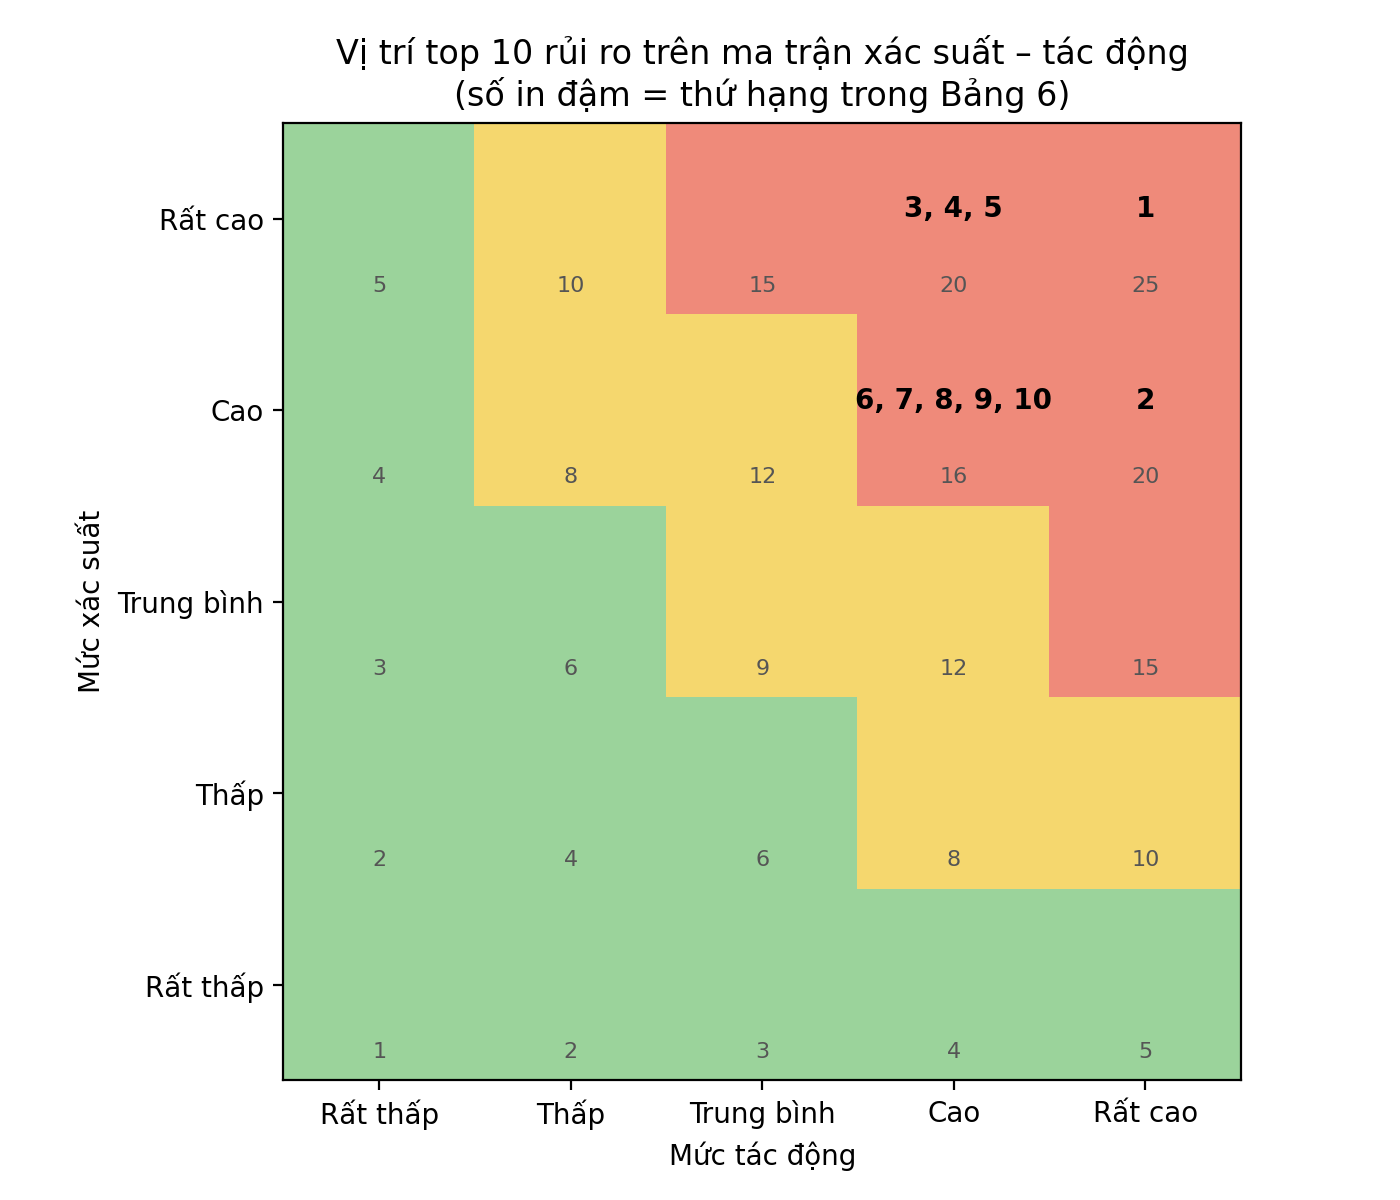
\includegraphics[width=0.72\textwidth]{ma_tran_pim_top10.png}
\caption{Vị trí 10 rủi ro hàng đầu trên ma trận xác suất -- tác động (vẽ lại từ Bảng 6 trong~\cite{kassem2022})}
\label{fig:pim}
\end{figure}

\textbf{So sánh RII và PIM.} Hai công cụ dùng chung đầu vào nhưng trả lời hai câu hỏi khác nhau. RII cho ra một con số liên tục để \emph{xếp hạng}. PIM cho ra một \emph{vùng} để chọn chiến lược ứng phó. Vì PIM chỉ có 5 mức trên mỗi trục, nhiều rủi ro rơi vào cùng một ô: trong Hình~\ref{fig:pim}, năm rủi ro xếp hạng 6 đến 10 cùng nằm ở ô (Cao, Cao) và không phân biệt được với nhau. Ngược lại, RII phân biệt được các yếu tố chỉ chênh nhau vài phần nghìn, nhưng không cho biết nên ứng phó thế nào. Một điểm đáng chú ý là thứ hạng theo hai cách không trùng nhau. Theo RII, ``chính phủ bất ổn'' đứng đầu~\cite{kassem2022}, nhưng yếu tố này không có trong top 10 của ma trận. Chương~\ref{chuong:tai-hien} sẽ kiểm tra lại sự nhất quán giữa hai bảng này.

\section{Mô hình phương trình cấu trúc (SEM)}
\label{sec:sem}

\subsection{Biến tiềm ẩn và biến quan sát}

Nhiều khái niệm trong quản lý dự án không đo trực tiếp được, chẳng hạn ``rủi ro từ phía chủ đầu tư'' hay ``mức độ thành công của dự án''. Những khái niệm như vậy gọi là \textbf{biến tiềm ẩn} (latent variable, construct). Ta chỉ đo được chúng gián tiếp qua các câu hỏi cụ thể gọi là \textbf{biến quan sát} (indicator). Ví dụ, biến tiềm ẩn ``rủi ro chủ đầu tư'' (CL) trong bài báo được đo qua sáu câu CL1--CL6, trong đó CL1 là ``chậm ra quyết định''.

Mô hình phương trình cấu trúc (SEM) là kỹ thuật thống kê đa biến cho phép ước lượng đồng thời hai loại quan hệ~\cite{hair2022primer}:
\begin{itemize}
  \item \textbf{Mô hình đo lường} (mô hình ngoài, outer model): quan hệ giữa mỗi biến tiềm ẩn và các câu hỏi đo nó.
  \item \textbf{Mô hình cấu trúc} (mô hình trong, inner model): quan hệ giữa các biến tiềm ẩn với nhau. Đây chính là các giả thuyết nghiên cứu.
\end{itemize}

Biến tiềm ẩn chỉ đóng vai trò giải thích (không bị biến nào khác tác động) gọi là \textbf{biến ngoại sinh}. Biến tiềm ẩn bị các biến khác tác động gọi là \textbf{biến nội sinh}. Trong bài báo, các nhóm rủi ro là biến ngoại sinh, còn ``ảnh hưởng tới thành công dự án'' là biến nội sinh.

\subsection{Hai cách tiếp cận: CB-SEM và PLS-SEM}

Có hai họ phương pháp ước lượng SEM. CB-SEM (dựa trên hiệp phương sai) tìm bộ tham số sao cho ma trận hiệp phương sai do mô hình tạo ra gần nhất với ma trận hiệp phương sai của dữ liệu, nên phù hợp để \emph{kiểm định một lý thuyết} đã có. PLS-SEM (bình phương tối thiểu riêng phần) tìm bộ tham số sao cho phần phương sai được giải thích của các biến nội sinh là lớn nhất, nên thiên về \emph{giải thích và dự báo}~\cite{hair2022primer,hair2019report}. Bảng~\ref{tab:cb-pls} so sánh hai cách tiếp cận.

\begin{table}[H]
\centering
\caption{So sánh CB-SEM và PLS-SEM (tổng hợp từ~\cite{hair2022primer,hair2019report})}
\label{tab:cb-pls}
\begin{tabularx}{\textwidth}{@{}p{3.6cm}XX@{}}
\toprule
\textbf{Tiêu chí} & \textbf{CB-SEM} & \textbf{PLS-SEM} \\
\midrule
Mục tiêu & Kiểm định, xác nhận lý thuyết & Giải thích phương sai, dự báo, phát triển lý thuyết \\
Giả định phân phối & Cần phân phối chuẩn đa biến & Không cần (phi tham số) \\
Cỡ mẫu & Thường cần lớn (vài trăm trở lên) & Chạy được với mẫu nhỏ hơn \\
Độ phức tạp mô hình & Khó hội tụ khi nhiều biến & Xử lý tốt mô hình nhiều biến, nhiều bậc \\
Độ phù hợp toàn cục & Có ($\chi^2$, CFI, RMSEA\ldots) & Không có chỉ số được thừa nhận rộng rãi \\
Phần mềm phổ biến & AMOS, LISREL, Mplus & SmartPLS, gói seminr (R) \\
\bottomrule
\end{tabularx}
\end{table}

Bài báo chọn PLS-SEM với ba lý do: dữ liệu Likert không có phân phối chuẩn, mô hình phức tạp (51 câu hỏi, 13 nhóm, 2 bậc) và mục tiêu là xác định các yếu tố có ảnh hưởng lớn nhất~\cite{kassem2022}. Lựa chọn này phù hợp với khuyến nghị của Hair và cộng sự~\cite{hair2019report}.

\section{Phương pháp PLS-SEM}
\label{sec:pls-sem}

\subsection{Thuật toán ước lượng}

Thuật toán PLS-SEM ước lượng điểm của mỗi biến tiềm ẩn $Y_j$ như một tổ hợp tuyến tính có trọng số của các câu hỏi đo nó, rồi chạy hồi quy giữa các biến tiềm ẩn. Các trọng số được tìm bằng cách lặp~\cite{hair2022primer,tenenhaus2005}:
\begin{enumerate}
  \item \textbf{Khởi tạo:} gán mọi trọng số ngoài $w_{kj} = 1$.
  \item \textbf{Xấp xỉ ngoài:} tính điểm biến tiềm ẩn từ các câu hỏi rồi chuẩn hóa:
  \begin{equation}
  Y_j = \sum_{k} w_{kj}\, x_{kj}
  \label{eq:xap-xi-ngoai}
  \end{equation}
  \item \textbf{Xấp xỉ trong:} tính một ước lượng khác của mỗi biến tiềm ẩn từ các biến tiềm ẩn kề với nó trong mô hình cấu trúc:
  \begin{equation}
  Z_j = \sum_{i \neq j} e_{ji}\, Y_i
  \label{eq:xap-xi-trong}
  \end{equation}
  trong đó $e_{ji}$ là trọng số trong, tính theo lược đồ đường dẫn (path weighting scheme).
  \item \textbf{Cập nhật trọng số ngoài:} với mô hình đo lường kết quả (reflective, Mode A), trọng số mới là hiệp phương sai giữa câu hỏi và ước lượng trong, $w_{kj} = \operatorname{cov}(x_{kj}, Z_j)$.
  \item \textbf{Lặp lại} bước 2--4 cho tới khi tổng thay đổi của các trọng số nhỏ hơn ngưỡng (SmartPLS mặc định $10^{-7}$).
  \item \textbf{Ước lượng cuối:} loading $\lambda_{kj} = \operatorname{corr}(x_{kj}, Y_j)$. Hệ số đường dẫn $\beta$ là hệ số hồi quy OLS của mỗi biến nội sinh theo các biến tác động lên nó.
\end{enumerate}

\subsection{Bootstrapping và kiểm định giả thuyết}

PLS-SEM không giả định phân phối, nên không có công thức sai số chuẩn như hồi quy thông thường. Sai số chuẩn được ước lượng bằng \textbf{bootstrapping}: rút ngẫu nhiên có hoàn lại $B$ mẫu con (thường $B = 5000$), mỗi mẫu cùng cỡ $n$ với mẫu gốc, chạy lại thuật toán trên từng mẫu để có $B$ giá trị $\hat\beta^{(b)}$. Sai số chuẩn là độ lệch chuẩn của các giá trị đó, và thống kê kiểm định là:
\begin{equation}
t = \frac{\hat\beta}{SE(\hat\beta)}, \qquad SE(\hat\beta) = \sqrt{\frac{1}{B-1}\sum_{b=1}^{B}\left(\hat\beta^{(b)} - \bar{\beta}\right)^2}
\label{eq:bootstrap}
\end{equation}
Với kiểm định hai phía ở mức ý nghĩa 5\%, giả thuyết được ủng hộ khi $|t| > 1{,}96$ (tương ứng $p < 0{,}05$).

\subsection{Đánh giá mô hình đo lường}

Mô hình đo lường kết quả được đánh giá qua độ tin cậy, giá trị hội tụ và giá trị phân biệt~\cite{hair2019report,hair2022primer}:
\begin{itemize}
  \item \textbf{Loading} $\lambda$: mức độ câu hỏi phản ánh biến tiềm ẩn. Ngưỡng $\lambda \geq 0{,}708$, vì khi đó $\lambda^2 \geq 0{,}5$, tức biến tiềm ẩn giải thích ít nhất một nửa phương sai của câu hỏi.
  \item \textbf{Độ tin cậy tổng hợp} (CR):
  \begin{equation}
  CR = \frac{\left(\sum_{k=1}^{K}\lambda_k\right)^2}{\left(\sum_{k=1}^{K}\lambda_k\right)^2 + \sum_{k=1}^{K}\left(1 - \lambda_k^2\right)}
  \label{eq:cr}
  \end{equation}
  Ngưỡng từ 0,70 đến 0,95. Giá trị trên 0,95 là dấu hiệu các câu hỏi trùng lặp nhau.
  \item \textbf{Phương sai trung bình được trích} (AVE), đo giá trị hội tụ:
  \begin{equation}
  AVE = \frac{1}{K}\sum_{k=1}^{K}\lambda_k^2
  \label{eq:ave}
  \end{equation}
  Ngưỡng $AVE \geq 0{,}5$.
  \item \textbf{Giá trị phân biệt}: các biến tiềm ẩn phải thực sự khác nhau. Tiêu chí Fornell--Larcker~\cite{fornell1981} yêu cầu $\sqrt{AVE_j}$ lớn hơn tương quan của biến $j$ với mọi biến tiềm ẩn khác. Henseler và cộng sự~\cite{henseler2015} chỉ ra tiêu chí này thường không phát hiện được vấn đề và đề xuất tỷ số HTMT (trung bình tương quan giữa các câu hỏi khác nhóm chia cho trung bình tương quan giữa các câu hỏi cùng nhóm), với ngưỡng 0,85, hoặc 0,90 với các khái niệm gần nhau.
\end{itemize}

\subsection{Đánh giá mô hình cấu trúc}

\begin{itemize}
  \item \textbf{Hệ số xác định} $R^2$: tỷ lệ phương sai của biến nội sinh được các biến tác động lên nó giải thích. Theo Hair và cộng sự~\cite{hair2019report}, các mức 0,75 / 0,50 / 0,25 tương ứng mạnh / trung bình / yếu. Chin~\cite{chin1998} dùng các mức 0,67 / 0,33 / 0,19.
  \item \textbf{Quy mô tác động} $f^2$: mức giảm $R^2$ khi bỏ một biến ngoại sinh khỏi mô hình,
  \begin{equation}
  f^2 = \frac{R^2_{co} - R^2_{bo}}{1 - R^2_{co}}
  \label{eq:f2}
  \end{equation}
  với các mức 0,02 / 0,15 / 0,35 tương ứng nhỏ / trung bình / lớn~\cite{cohen1988}.
  \item \textbf{Mức liên quan dự báo} $Q^2$, tính bằng thủ tục blindfolding: lần lượt che một phần dữ liệu, dự báo lại phần bị che rồi so sánh,
  \begin{equation}
  Q^2 = 1 - \frac{SSE}{SSO}
  \label{eq:q2}
  \end{equation}
  trong đó $SSE$ là tổng bình phương sai số dự báo và $SSO$ là tổng bình phương các giá trị quan sát, bằng $n \times K$ với $K$ là số câu hỏi của biến. Mô hình có khả năng dự báo khi $Q^2 > 0$.
  \item \textbf{Chỉ số phù hợp} GoF do Tenenhaus và cộng sự~\cite{tenenhaus2005} đề xuất:
  \begin{equation}
  GoF = \sqrt{\overline{AVE} \times \overline{R^2}}
  \label{eq:gof}
  \end{equation}
  Bài báo dùng ngưỡng 0,36 để kết luận mô hình phù hợp. Tuy nhiên Henseler và Sarstedt~\cite{henseler2013} đã chỉ ra GoF không phân biệt được mô hình đúng với mô hình sai, và Hair và cộng sự~\cite{hair2019report} khuyến nghị không dùng chỉ số này.
\end{itemize}

\section{Mô hình nghiên cứu của bài báo}
\label{sec:mo-hinh}

Mô hình của bài báo (Hình~\ref{fig:mo-hinh}) là một mô hình \textbf{hai bậc}. Ở bậc 1, 51 câu hỏi đo 13 nhóm rủi ro. Ở bậc 2, 13 nhóm này được gom thành hai khái niệm tổng quát hơn: \emph{rủi ro nội bộ} gồm 7 nhóm (chủ đầu tư, nhà thầu, tư vấn, khả thi và thiết kế, đấu thầu và hợp đồng, nguồn lực và vật tư, quản lý dự án) và \emph{rủi ro bên ngoài} gồm 6 nhóm (kinh tế, chính trị, người dân địa phương, môi trường và an toàn, an ninh, bất khả kháng). Hai khái niệm bậc 2 cùng tác động lên biến nội sinh \emph{ảnh hưởng của rủi ro tới thành công dự án}, đo bằng năm hậu quả EF1--EF5.

\begin{figure}[H]
\centering
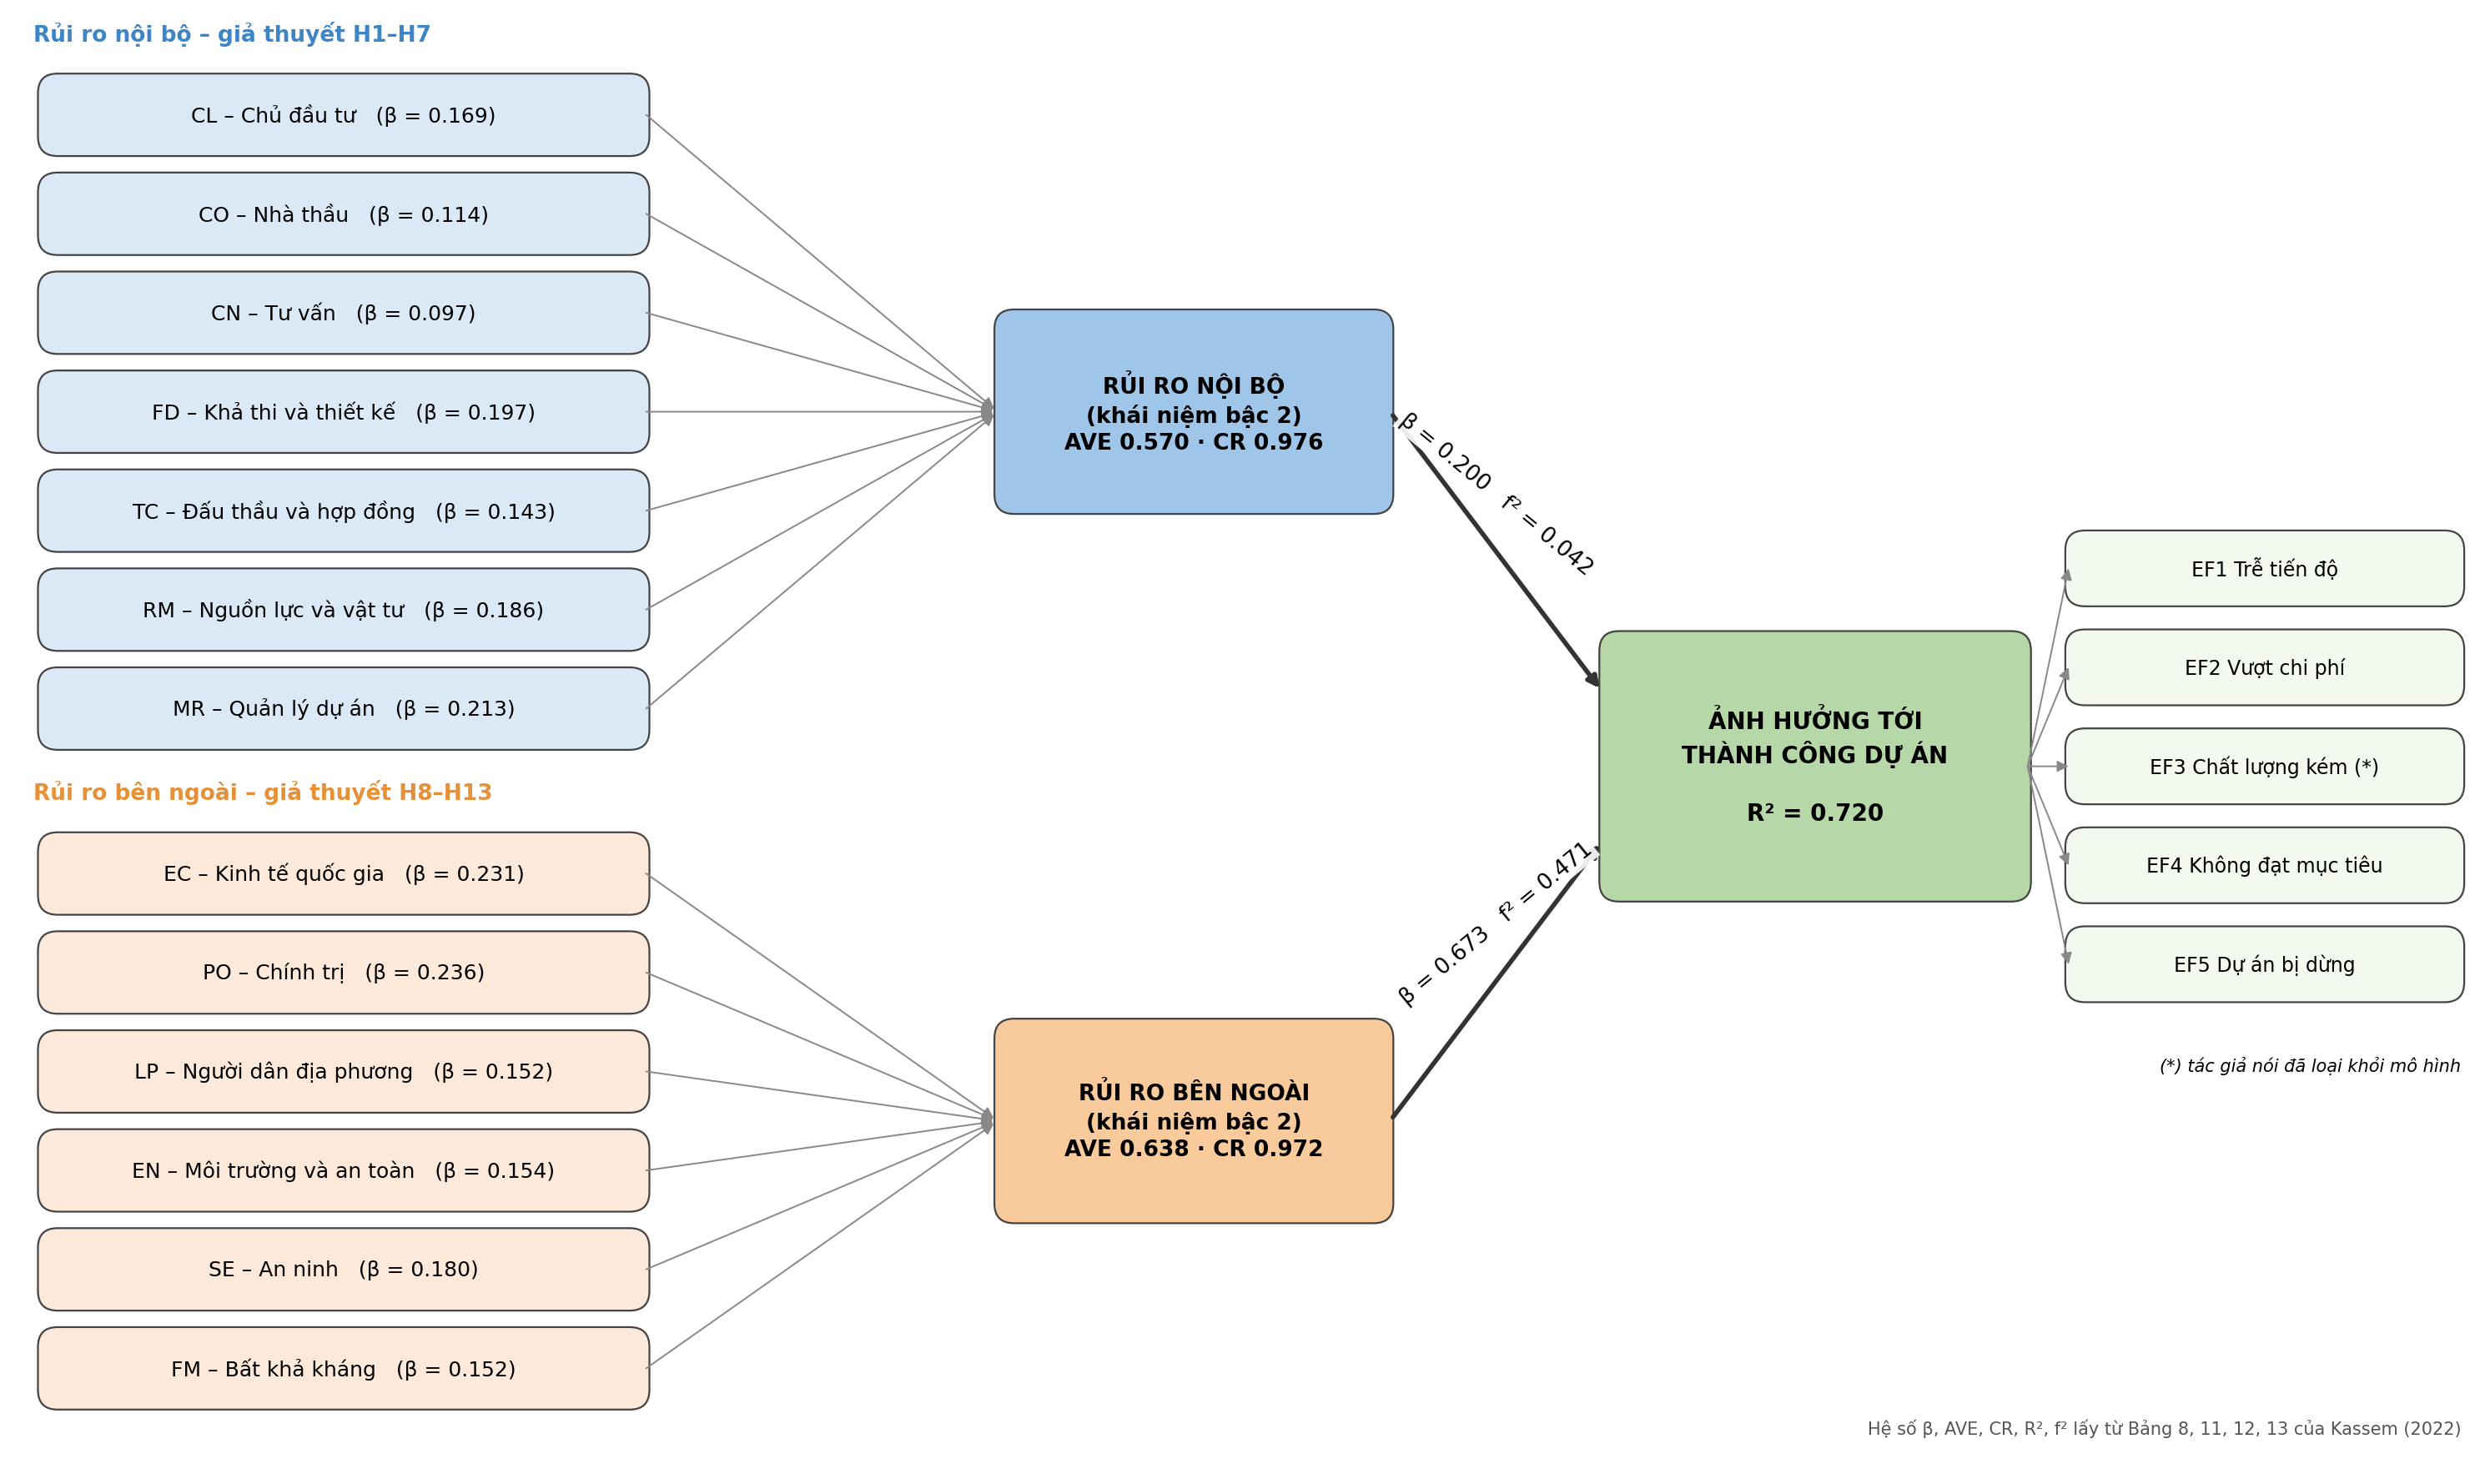
\includegraphics[width=\textwidth]{mo_hinh_nghien_cuu.png}
\caption{Mô hình nghiên cứu hai bậc và các hệ số do bài báo công bố (vẽ lại từ~\cite{kassem2022})}
\label{fig:mo-hinh}
\end{figure}

Tác giả phát biểu 13 giả thuyết H1--H13 có chung dạng ``nhóm rủi ro X ảnh hưởng tới thành công của dự án xây dựng'', mỗi giả thuyết ứng với một nhóm. Phần thảo luận còn nhắc tới H14 và H15 mà không định nghĩa. Căn cứ vào ngữ cảnh, đó là hai đường dẫn từ rủi ro nội bộ và rủi ro bên ngoài tới thành công dự án.

Khi đọc mô hình cần lưu ý hai điểm:
\begin{enumerate}
  \item Biến nội sinh được đo bằng các \emph{hậu quả xấu}: điểm càng cao thì dự án càng chịu nhiều tác động tiêu cực. Vì vậy hệ số $\beta$ dương nghĩa là rủi ro càng lớn thì dự án càng \emph{kém} thành công.
  \item Trong mô hình hai bậc, các nhóm bậc 1 không nối trực tiếp tới biến nội sinh mà đi qua khái niệm bậc 2. Có nhiều cách ước lượng loại mô hình này, như lặp chỉ báo (repeated indicators) hay hai giai đoạn (two-stage), và mỗi cách cho kết quả khác nhau~\cite{sarstedt2019hoc}. Bài báo không nói đã dùng cách nào, nên không rõ 13 hệ số $\beta$ của từng nhóm được tính ra sao. Chương~\ref{chuong:tai-hien} sẽ phân tích kỹ hơn điểm này.
\end{enumerate}

\section{Ứng dụng, ưu điểm, hạn chế và xu hướng}
\label{sec:danh-gia-pp}

\subsection{Ứng dụng}

PLS-SEM được dùng nhiều trong marketing, hệ thống thông tin (ví dụ các mô hình chấp nhận công nghệ), quản trị chiến lược, và ngày càng phổ biến trong quản lý xây dựng~\cite{hair2022primer}. Trong quản lý dự án, phương pháp này thường được dùng để mô hình hóa nguyên nhân chậm tiến độ, vượt chi phí và rủi ro~\cite{kassem2022}. Ngay trong lĩnh vực hệ thống thông tin, đã có nghiên cứu dùng SEM để phân tích ảnh hưởng của mức độ không chắc chắn và quản lý rủi ro lên kết quả của dự án phát triển hệ thống thông tin (tài liệu [15] trong~\cite{kassem2022}).

\subsection{Ưu điểm}

\begin{itemize}
  \item Không đòi hỏi phân phối chuẩn, phù hợp với dữ liệu khảo sát thang Likert.
  \item Chạy được mô hình nhiều biến, nhiều bậc mà CB-SEM khó hội tụ.
  \item Cho ra điểm số cụ thể của từng biến tiềm ẩn, dùng được cho các phân tích tiếp theo.
  \item Kết hợp được với RII và PIM: RII và PIM trả lời câu hỏi ``rủi ro nào quan trọng'', còn PLS-SEM trả lời ``nhóm rủi ro nào ảnh hưởng tới kết quả dự án và mạnh đến đâu''.
\end{itemize}

\subsection{Hạn chế}

\begin{itemize}
  \item Với mô hình đo lường kết quả, PLS-SEM có xu hướng ước lượng loading cao hơn và hệ số đường dẫn thấp hơn giá trị thật. Phiên bản PLS nhất quán (PLSc) được đề xuất để khắc phục~\cite{dijkstra2015}.
  \item Không có chỉ số phù hợp toàn cục được thừa nhận. Việc dùng GoF như bài báo không còn được khuyến nghị~\cite{henseler2013}.
  \item Kết quả phụ thuộc vào chất lượng dữ liệu khảo sát. Nếu người trả lời chấm theo một cảm nhận chung (ví dụ ``mọi thứ ở Yemen đều rủi ro''), các nhóm sẽ tương quan cao với nhau và giá trị phân biệt bị ảnh hưởng.
  \item Mô hình chỉ cho thấy mối liên hệ thống kê. Dữ liệu cắt ngang từ một lần khảo sát không đủ để khẳng định quan hệ nhân quả theo nghĩa chặt chẽ.
\end{itemize}

\subsection{Xu hướng}

\begin{itemize}
  \item \textbf{Đánh giá khả năng dự báo ngoài mẫu} bằng PLSpredict, thay cho $Q^2$ tính trong mẫu~\cite{shmueli2019}.
  \item \textbf{Dùng HTMT} thay cho Fornell--Larcker làm tiêu chí giá trị phân biệt chính~\cite{henseler2015}.
  \item \textbf{Chuẩn hóa cách xây dựng mô hình bậc cao}~\cite{sarstedt2019hoc}.
  \item \textbf{Công cụ mã nguồn mở} như gói seminr trên R giúp người khác tái hiện được kết quả~\cite{hair2021workbook}. Điều này đặc biệt quan trọng khi dữ liệu gốc không được công bố, như trường hợp của bài báo này.
\end{itemize}
